
\documentclass{sig-alternate}
\usepackage{balance,array}
\usepackage[bf]{subfigure}

\let\proof\relax
\let\endproof\relax

\usepackage{color, times, mathptmx, amsmath, amssymb, amsthm, verbatim, 
  mdwlist, graphicx, footnote, multirow, xspace, tikz, colortbl,cite}

\DeclareMathAlphabet{\mathcal}{OMS}{cmsy}{m}{n}
\let\footnotesize\small

%\usepackage{draftwatermarktop, draftwatermarkbottom}
\usepackage{algorithm}% http://ctan.org/pkg/algorithms

\usepackage[noend]{algpseudocode}% http://ctan.org/pkg/algorithmicx

% Franklin, Alvaro, Conway, Venkataraman, Panda

\setlength{\parskip}{3ex plus 2ex minus 2ex}

\algrenewcommand{\alglinenumber}[1]{\small#1:}

\theoremstyle{definition}
\setlength{\textfloatsep}{1em}% Remove \textfloatsep

\renewcommand\topfraction{0.85}
\renewcommand\bottomfraction{0.85}
\renewcommand\textfraction{0.1}
\renewcommand\floatpagefraction{0.85}

\newtheorem{invariant}{Invariant}
\newtheorem{lemma}{Lemma}

\makeatletter
\def\thm@space@setup{\thm@preskip=.5em
\thm@postskip=.5em}
\makeatother

\newtheorem{definition}{Definition}
\newtheorem{theorem}{Theorem}
\newtheorem{myproof}{Proof}
\newtheorem{claim}{Claim}

\theoremstyle{remark}

\newtheorem{remark}{Remark}

\usepackage{scrextend}
\usepackage[hyphens]{url}

\usepackage[hidelinks]{hyperref}
\usepackage{breakurl}

\newcommand{\commentt}[1]{{\small\texttt{#1}}}

\newcommand{\example}[1]{{\vspace{.25em}\noindent\textbf{#1.} }}
\newcommand{\miniheadnostop}[1]{{\vspace{.4em}\noindent\textit{#1} }}
\newcommand{\minihead}[1]{{\vspace{.4em}\noindent\textbf{#1.} }}
\newcommand{\miniheadnopd}[2]{{\vspace{.4em}\noindent\textbf{#1}\hspace{.5em}{#2}\vspace{.4em} }}
\newcommand{\minidef}[1]{{\vspace{.25em}\noindent\textit{#1} }}

\newcommand{\pbnote}[1]{{\color{red}{#1 ---P.B.}}}

\newcommand{\ttf}[1]{\texttt{#1}\xspace}

\newcommand{\cfree}{coordination-free\xspace}
\newcommand{\cfreedom}{coordination-freedom\xspace}


\newcommand{\fullnameconfluence}{invariant confluence\xspace}
\newcommand{\iconfluent}{$\mathcal{I}$-confluent\xspace}
\newcommand{\iconfluence}{$\mathcal{I}$-confluence\xspace}



\newcommand{\ramp}{ANON\xspace}


\newcommand{\dpc}{\ttf{D-2PC}}
\newcommand{\cpc}{\ttf{C-2PC}}


\hyphenation{da-ta-base}

\newcommand{\rapl}{\ttf{RAMP-L}}
\newcommand{\raps}{\ttf{RAMP-S}}
\newcommand{\rapb}{\ttf{RAMP-B}}

\newcommand{\lwlr}{\ttf{LWLR}}
\newcommand{\lwsr}{\ttf{LWSR}}
\newcommand{\lwnr}{\ttf{LWNR}}
\newcommand{\nwnr}{\ttf{NWNR}}
\newcommand{\mstr}{\ttf{MSTR}}

\usepackage{etoolbox}
\newcommand{\zerodisplayskips}{%
  \setlength{\abovedisplayskip}{4pt}
  \setlength{\belowdisplayskip}{4pt}
  \setlength{\abovedisplayshortskip}{4pt}
  \setlength{\belowdisplayshortskip}{4pt}}
\appto{\normalsize}{\zerodisplayskips}
\appto{\small}{\zerodisplayskips}
\appto{\footnotesize}{\zerodisplayskips}

\usepackage[T1]{fontenc}
\renewcommand{\ttdefault}{fi4}

\newenvironment{myitemize}
{
  \vspace{-.4em}
    \begin{list}{$\bullet$ }{}
        \setlength{\topsep}{0em}
        \setlength{\parskip}{0pt}
        \setlength{\partopsep}{0pt}
        \setlength{\parsep}{0pt}         
        \setlength{\itemsep}{.25em} 
        \setlength{\itemindent}{0em}
}
{
    \end{list} 
    \vspace{-.4em}
}

\newenvironment{introenumerate}
{

   \vspace{-.5em}
   \newcounter{qdcounter}
    \begin{list}{\arabic{qdcounter}.~}{\usecounter{qdcounter}\leftmargin=1em}
        \setlength{\topsep}{0em}
        \setlength{\parskip}{0pt}
        \setlength{\partopsep}{0pt}
        \setlength{\parsep}{0pt}         
        \setlength{\itemsep}{.25em} 
        \setlength{\itemindent}{0em}
}
{
    \end{list} 
    \vspace{-.5em}
}


\usepackage[leftmargin=0em]{quoting}

\begin{document}
%
% --- Author Metadata here ---
\conferenceinfo{XXX}{YYY}
%\CopyrightYear{2007} % Allows default copyright year (20XX) to be over-ridden - IF NEED BE.
%\crdata{0-12345-67-8/90/01}  % Allows default copyright data (0-89791-88-6/97/05) to be over-ridden - IF NEED BE.
% --- End of Author Metadata ---

\title{Coordination-Avoiding Database Systems}

%{\author{Peter Bailis, Alan Fekete{\fontsize{12}{14}$^\dagger$}, Ali Ghodsi, Joseph M. Hellerstein, Ion Stoica \\{\affaddr{UC Berkeley and {\fontsize{12}{14}$^\dagger$}University of Sydney}}}}
\maketitle



\begin{abstract}
Concurrent access to shared state results in a fundamental trade-off
between coordination---surfacing in the form of availability, latency,
and scalability---and application-level consistency, or semantic
guarantees for end users. Traditional mechanisms such as serializable
transactions are sufficient to ensure application-level consistency
but require synchronous coordination, while weaker mechanisms in turn
may sacrifice consistency for asynchronous coordination and greater
scale. In this paper, we identify a necessary and sufficient condition
for achieving \cfree execution without violating application-level
consistency: \fullnameconfluence. By explicitly considering
application-level invariants, \fullnameconfluence analysis allows
databases to coordinate between operations only when anomalies that
might violate invariants are possible. This provides a formal basis
for coordination-avoiding database systems, which coordinate only when
it is provably necessary to do so. We demonstrate the utility of
\fullnameconfluence analysis via analysis of a subset of SQL,
application analysis, and a proof-of-concept database prototype.
\end{abstract}



\section{Introduction}
\label{sec:intro}

% coordination-freedom provides scalability

Minimizing coordination enables high performance, scalable database
designs. Coordination---informally, the requirement that concurrently
executing operations communicate or otherwise stall in order to
complete---is expensive: it prohibits parallel execution, limits
availability in the presence of partial failure, and requires
potentially high latency as communication costs increase (e.g.,
wide-area networks)~\cite{hat-vldb,gilbert-cap}. A system without
synchronous coordination---that is \textit{\cfree}---can scale
indefinitely: adding more query processing capacity (e.g., servers)
does not incur additional overhead as queries can execute
independently. In contrast with scale-out across multiple data items
(as in ``shared-nothing''
designs~\cite{bernstein-book,f1,spanner,pnuts,hstore}), \cfreedom
allows scale-out even at the granularity of a single contended data
item and ensures both high availability~\cite{gilbert-cap} and low
latency execution~\cite{pacelc}.

% serializability is traditional answer to correctness, but requires
% coordination

Unfortunately, traditional approaches to maintaining correct data
during concurrent access are at odds with the goal of \cfreedom. The
serializable transaction concept provides concurrent operations
(transactions) with the illusion of executing in some serial
order~\cite{bernstein-book}. Serializability is \textit{sufficient} to
guarantee application-level consistency: if individual transactions
maintain correct application state, then a serially ordered execution
will not violate correctness~\cite{gray-virtues}. However,
serializability incurs a steep coordination cost: at the level of
reads and writes, any write potentially conflicts with any other read
or write to the same item, requiring coordination for safe
execution~\cite{hat-vldb,davidson-survey}. A proliferation of
alternative data management solutions (e.g., ``NoSQL'') offer greater
scalability by foregoing such strong
semantics~\cite{dynamo,optimistic} but, in practice, require end-users
to make ad-hoc decisions to determine when weakened semantics are
acceptable for applications~\cite{consistency-borders}.

% which anomalies matter depends on application; think about
% invariants instead, use to identify necessary and sufficient
% condition

In this paper, we seek an alternative: coordination-avoiding
concurrency control strategies that coordinate only when it is
provably \textit{necessary} for correctness. For arbitrary
applications, \textit{anomalies} resulting from non-serializable
execution~\cite{adya-isolation} may compromise application
correctness: for example, multiple users might be assigned the same
username, or, in a classic example, a bank account balance might be
negative. Our task is to categorize and only prevent those anomalies
that can violate application-level consistency---without requiring
users to reason about low-level isolation models~\cite{hat-vldb}
themselves. This requires more information about applications than
traditional~\cite{bernstein-book,gray-virtues} (but not
all~\cite{eswaran-consistency,korth-serializability,decomp-semantics,garciamolina-semantics,activedb-book,ic-survey,ic-survey-two})
transaction models: users will specify \textit{invariants} (i.e.,
integrity constraints)~\cite{traiger-tods}, or predicates representing
application-level correctness criteria that should always hold true
across database state(s). For example, users might inform the database
that usernames should be unique and that each customer should belong
to a bank branch.

To provide a formal basis for coordination-avoidance, we develop a
necessary and sufficient condition for \cfree execution under a given
set of invariants, called \textit{invariant confluence}. This
\iconfluence formalizes---at an application level---which operations
can be safely executed independently and in parallel and subsequently
``merged'' into consistent database state. We prove that a database
system can maintain invariants during \cfree, available, and
convergent operation if and only if the invariants are
\iconfluent. Accordingly, \iconfluence analysis can capture the
potential scalability of a given application: if an application passes
the \iconfluence test, it can be executed without coordination. If an
application fails the test, it will (provably) \textit{have} to
coordinate in order to guarantee correctness. This provides the
foundation for \textit{coordination-avoiding} database designs that
coordinate only when required. As we discuss in
Section~\ref{sec:relatedwork}, our core results marry concepts from
rule-based rewriting systems~\cite{obs-confluence,termrewriting},
distributed computing~\cite{herlihy-apologizing,gilbert-cap,hat-vldb},
and many prior database
concepts~\cite{activedb-book,ic-survey,ic-survey-two} such as
semantics-based concurrency
control~\cite{sdd1,decomp-semantics,badrinath-semantics,garciamolina-semantics,korth-serializability,atomictransactions,weihl-thesis},
in the context of (logically) replicated state.

% many workloads are amenable to cfree execution! the following ICs
% are actually okay. but if not, here's the cost.

We subsequently apply our \iconfluence coordination analysis to
existing applications and quantify the costs of
coordination. Specifically, we demonstrate that many common integrity
constraints are indeed achievable without coordination, including
forms of foreign key constraints, unique value generation, and
row-level check constraints. In contrast, others, like unique value
checks and sequence number generation do not. We apply this analysis
to existing benchmarks to determine their required degree of
coordination: surprisingly, many are executable without
coordination. As a case study, we focus on the TPC-C
benchmark~\cite{tpcc}, which has seen substantial popularity in the
database community as a gold standard for new concurrency control
algorithms~\cite{abadi-vll,jones-dtxn,schism,calvin,hstore}. We show
that, in fact, ten of twelve of TPC-C's integrity constraints are
\iconfluent and, more importantly, compliant TPC-C can be implemented
without synchronous coordination across servers. As a proof of
concept, we scale a simple coordination-avoiding database prototype
linearly, to over $1.8M$ New-Order transactions per second on a
$100$-node EC2 cluster. We also discuss other applications and
demonstrate the costs of coordination by analyzing upper bounds on
throughput due to to atomic commitment overhead.

While our results are not comprehensive, they provide a formal but
pragmatic grasp on the trade-off between coordination and
application-level consistency. We accordingly view this work as the
first step in revisiting core database concepts like query
optimization, failure recovery, and data layout in light of
coordination avoidance and increased knowledge of application-level
semantics.





\section{Coordination and Consistency}
\label{sec:motivation}

% application-level consistency is key requirement

As repositories for application state, databases are tasked with the
challenging goals of maintaining correct, durable data despite
concurrency, failures, and, often,
distribution~\cite{bernstein-book}. Core to the utility of a database
system is its ability to maintain application data that is
\textit{consistent}---that is, data that is well-formed according to
application semantics~\cite{gray-virtues}. By entrusting databases
with their data, applications are freed from the requirement to
manually manage this correctness. Maintaining consistency inherently
requires reasoning about and often controlling concurrent access to
data: in this section, we discuss this trade-off and describe classic,
conservative approaches to maintaining consistency.

\minihead{A simple example} As a motivating example running throughout
this paper, we consider a simple payroll application managing
information about employees and departments. We specifically consider
three aspects of the payroll application:
\begin{myitemize}
\item\textbf{Employee IDs:} Employees are assigned ID numbers that
  should be unique with respect to all other assigned IDs (i.e., a
  primary key constraint).
  \item\textbf{Departments:} Employees should belong to exactly one
  department (i.e., a foreign key constraint). Employees can switch
  departments by updating their department assignment.
\item\textbf{Salaries:} Employees have salaries, and no employee
  should have salary greater than $\$50,000$.
\end{myitemize}
A database supporting the payroll application will have to be careful
in managing correctness as multiple users concurrently access the
database state. For example, if Stan is assigned ID number $5$ and
Mary is simultaneously assigned ID number $5$, then the database
consistency will be compromised. On the other hand, properties like
the department constraint are easier to maintain. For example,
simultaneously adding Stan and Mary to the Engineering department is
safe. Effectively, some combinations of transactions and invariants
appear unsafe without coordination between concurrent operations,
whereas others appear to be resilient to independent access and
update.

A primary goal of this paper is to formalize this trade-off and state
a general property for deciding whether or not coordination is
required. More succinctly, we will answer the question: when does
correct transaction processing require synchronous coordination?

% traditional programmability: serializability; isolation is means
% towards achieving consistency

\minihead{Transactions and Isolation} The ACID transaction concept
pioneered by Jim Gray and System R relieved programmers of the
requirement to explicitly specify their consistency constraints by
encouraging the use of serializable
transactions~\cite{gray-virtues}. Under serialiable isolation, the
execution of a set of transactions is equivalent to some serial
ordering between them~\cite{bernstein-book}. As long as each
transaction leaves the database in a consistent state, serializable
transactions ensure database consistency. Accordingly, traditional
database systems treat isolation between concurrently executing
transactions as a \textit{means} towards achieving application
consistency. Serializable transactions are a \textit{sufficient}
mechanism for ensuring consistency but are not strictly
\textit{necessary}: as a classic example due to Lamport in
1976~\cite{lamport-audit}, an ``audit'' transaction over shared bank
account balances need not observe serializable state as long as no
bank account balance it reads is negative.

% problem: serializability is actually pretty expensive; seen shift
% away from them

\minihead{Coordination costs} While serializability provides a
remarkably powerful and convenient abstraction, it is accompanied by a
hefty price tag: a requirement for
coordination~\cite{davidson-survey}. We formally define coordination
in Section~\ref{sec:model}, but, informally, we say that a database is
\textit{coordination-free} if each copy of shared database state can
can execute operations without contacting (and, therefore, possibly
stalling) other copies of state. This requirement has been captured in
the distributed systems community as \textit{availability}, or
``always-on'' operation: an available distributed system can perform
operations on any non-failed server, despite arbitrary communication
partitions between servers~\cite{gilbert-cap}. This also benefits
normal operation: to serve a request, a \cfree server need not contact
any others~\cite{pacelc}, so client requests can safely proceed in
parallel. In contrast, a system that requires coordination (e.g.,
provides serializability) faces unavailability in the presence of
network partitions and partial failures, and, during normal operation,
incurs higher latency due to communication delays~\cite{hat-vldb} and,
possibly, resource contention, unstable queuing effects~\cite{ladis},
deadlocks, and spurious
aborts~\cite{bernstein-book,gray-book,gray-virtues}.

% cost of coordination? unavailability, latency, stalls : focus on
% worst-case behavior yields average-case benefits

% benefit of coordination-freedom: infinite scalability

\minihead{Coordination and scalability} Most importantly,
coordination-freedom is intrinsic to scalable execution. A \cfree
system can scale without barriers: if the demands for a given resource
grow beyond that of a single computer, another computer can be added
to the system. The additional computer and the original (set of)
computer(s) need not synchronously coordinate, so adding more
computers results in a linear increase in capacity that can be
repeated indefinitely. While the term ``scalability'' is often abused,
coordination-freedom captures the essential property of a perfect
scale-out system, even for single-record operations.

% spectrum of models; actually infinitely many of them
% not necessarily even easy to program

\minihead{Alternative models} Given the costs of coordination, many
database designs and systems operators opt for weaker models that
offer higher performance, lower latency, and fewer aborts. On a
single-node database, these models are often in the form of ``weak
isolation'' such as Read Committed and Repeatable Read
isolation~\cite{adya-isolation}. Modern distributed databases offer a
range of models such as eventual consistency and regular register
semantics~\cite{hat-vldb}.\footnote{To prevent confusion, we will
  subsequently refer to distributed systems consistency models such as
  linearizability as \textit{isolation models} (or, more simply,
  \textit{models}) and reserve the use of \textit{consistency} for
  referring to application-level ``ACID'' consistency guarantees. This
  is largely a product of scope: in a system where an end-user
  application is not considered (e.g., the traditional distributed
  systems literature), ``consistency'' is indeed best defined
  according to reads and writes on opaque registers.}  Not all weaker
models are \cfree (e.g., Snapshot Isolation)~\cite{hat-vldb}, but all
expose end users to isolation \textit{anomalies}, or behavior that
could not have arisen in a serial execution.

Unfortunately, determining whether weak isolation (and, moreover,
which isolation model) is safe for a given application is
difficult. Anomalies are often expressed in terms of (in-)admissible
traces of reads and writes, and the distinctions between models are
often subtle~\cite{adya-isolation,isolation-semantics} and vary
between implementations~\cite{hat-vldb}. Users must manually translate
from low-level traces to specific application behaviors, an
error-prone and laborious process, particularly for the non-specialist
developer~\cite{consistency-borders}. In the words of one senior
database community member, foregoing serializability is tantamount to
``falling off a cliff.'' If a developer chooses an incorrect model,
she risks inconsistency or, alternatively, extraneous
coordination. More fundamentally, any choice she makes ties her
application implementation and database execution strategy to a fixed
isolation model, which may not maintain correctness as application
logic evolves or as multiple applications concurrently access shared
data. As a final concern, the proliferation of isolation models and
deployment of multiple systems to support varying performance and
isolation requirements (so-called ``Polyglot
Persistence'')~\cite{polyglot} hint that different operations---even
within a single application---need a \textit{combination} of
guarantees---one model does not fit all.

% dividing line: coordination---define them

% evidence for mixed models: polyglot persistence, adding support for
% CAS, basis for lock manager, etc.

\minihead{Correctness without coordination} We desire an alternative
that manages the trade-off between coordination and correctness while
reducing the tension between programmability and
performance. Applications should ideally execute with as little
coordination as possible, but non-serializable isolation anomalies can
and will result in inconsistency for arbitrary applications. We must
answer the question: given an application, which anomalies are
important? Rather than require application writers to manually
classify anomalies, we will instead formulate our criteria for
coordination in terms of application-level semantics. Given a set of
invariants describing application state (e.g., as part of the SQL
DDL), we will present a necessary and sufficient condition for
coordination-free execution. While this task requires some
formalization (Sections~\ref{sec:model},\ref{sec:bcc-theory}), we
demonstrate that it can yield pragmatic results both in languages like
SQL (Section~\ref{sec:bcc-practice}) and in real system deployments
(Section~\ref{sec:evaluation}).

% if you give up serializability, can't guarantee correctness in an
% arbitrary read/write model; users have to manage this trade-off for
% themselves

% here, consider a model where stored procedures are declared in
% advance, invariants are given to the database; goal will be to
% minimize synchronize coordination




\section{System Model}
\label{sec:model}

In this section, we present our model for transactions, invariants,
and coordination.

\minihead{Transactions} In this paper, we consider a set of users
accessing a shared database, which contains a versioned set of data
items. In our initial formulation, we will represent database state as
a bag of mutations (much like a write-ahead log~\cite{gray-book}), but
we will consider other, more pragmatic representations in
Section~\ref{sec:bcc-practice}; we assume that the database is
initially populated by an initial state $D_0$ (typically but not
necessarily empty). Users submit requests to the database in the form
of transactions, or groups of operations on data items that should be
executed together. Operations are often in the form of writes (which
add a new version to the database) or reads (which return a specific
version--or set of versions--from the database), but operations can
also operate on abstract data types, such as incrementing a counter
item or adding an item to a set item. When required---and certainly in
future sections of this paper---we will discuss specific operation
types, but, in general, we will not make any specific assumptions
about operations. A transaction can \textit{commit}, signaling
success, or \textit{abort}, signaling failure. As a pragmatic
guarantee (not strictly required for our formalism), we will require
that no transaction that commits observes the effects of aborted
transactions, and, if a transaction commits, its effects should
survive database failures. We define a transaction $T$ as a
transformation on state with side effects: $T: DB \rightarrow DB$.

\minihead{Invariants} We consider a model where users specify
invariants over arbitrary database state that determine whether a
given state is valid. For example, an invariant might express the
requirement that only one user in a database has a given ID.  We model
invariants as binary predicates on database state: $I: DB \rightarrow
\{true, false\}$. Given a set of invariants $I_s$, we say that the
database is \textit{valid} under $I_s$ if all invariants in $I_s$
evaluate to true and w require that $D_0$ be valid. Invariants
directly capture the notion of ACID
Consistency~\cite{bernstein-book,gray-virtues}.

\miniheadnostop{Why specify invariants?} The majority of existing work
on database concurrency control assumes a model whereby ``the [set of
  invariants] is generally not known to the system but is embodied in
the structure of the transaction''~\cite{traiger-tods}. Indeed,
Eswaran et al.'s seminal paper on the topic of consistency argues that
``a complete set of assertions would no doubt be as large as the
system istself''~\cite{eswaran-consistency}. Nevertheless, since 1976,
databases have introduced support for a finite set of
invariants~\cite{korth-serializability} in the form of primary key and
foreign key, uniqueness, and row-level ``check'' constraints. We
expand this set of invariants in Section~\ref{sec:bcc-practice} and
demonstrate that a small set of invariants adds sufficient expressive
power for many applications. It is possible to perform a conservative
analysis if a complete specification of invariants is missing, but
this will result in less useful results. One consolation is that,
unlike more general forms of axiomatic logic (e.g., Hoare-style
triples~\cite{decomp-semantics}), there is only one (set of)
invariant(s) defined per application that is applied for every
transaction.\vspace{.5em}

\minihead{Coordination} In this paper, we are concerned with
synchronization and coordination between multiple transactions. We
consider a system model with are multiple, replicated copies of
database state (\textit{replicas}) located in separate processes
(\textit{servers}) that can each respond to transaction requests.  To
prevent the system from unnecessarily aborting transactions in order
to provide a response, we say that a system provides
\textit{transactional availability} (liveness) if, whenever a client
executing a transaction $T$ can access at least one replica for each
item in $T$, $T$ eventually commits or otherwise aborts itself either
due to an \textit{abort} operation in $T$ or due to a violation of a
declared integrity constraint~\cite{hat-vldb}.\footnote{As Bailis et
  al. note~\cite{hat-vldb}, this definition precludes multi-server
  fault tolerance (durability). However, we can consider multi-server
  durability by extending this definition to include coordination with
  a finite number of servers. This does not greatly affect scalability
  because, as more replicas are added, coordination is constant.} We
say that a system is \textit{always valid} if all replicas always
contain valid state. To capture the effect of network partitions but
also to capture linear scalability, we say that a system is
\textit{\cfree} if replicas do not communicate in order to execute
transactions.

A primary goal in the remainder of this paper will be to understand
which combinations of invariants and transactions are achievable with
\cfreedom and availability. It is vacuously possible to maintain
``consistent'' database states by letting replicas diverge: in
distributed systems parlance, this guarantees \textit{safety} but not
\textit{liveness}~\cite{lamport-safety}. To ensure that replicas
eventually agree---reflecting a shared, common set of database
state---we will say that a system is \textit{convergent} if, in the
absence of new transactions and in the absence of indefinite
communication delays, all replicas eventually contain the same
state~\cite{vogels-defs}.

\miniheadnostop{A note on replicas} While most treatments of
distributed databases (including this one) often treat replicas as
individual servers, even a non-replicated database can provide users
with an interface that exposes multiple ``replicas''. In fact, a
multi-versioned database system~\cite{bernstein-book} effectively
provides each user with a copy of database state, even in the presence
of concurrent access and modification. The specific concurrency
control mechanism will dictate which transactions commit or not, but a
set of invariants and stored procedures that are achievable without
coordination can also be executed in parallel on a single-site system
without aborts due to concurrent operations or other isolation
anomalies.  In fact, our current prototype transaction model
(Section~\ref{sec:evaluation}) is based on multi-versioning and
snapshot reads (``logical replicas'') rather than actual multi-master
replication. Similar analogies can be drawn to general-purpose
optimistic methods (but not as much to lock-based schemes, which
largely limit concurrency), although we do not consider them here.



\section{Consistency sans Coordination}
\label{sec:bcc-theory}

With a system model and goals in hand, we now address the question:
when does transaction processing require synchronous coordination? The
answer depends not only on the transactions that a database may be
expected to perform and not only on the integrity constraints that the
database is required to maintain but instead depends on the
\textit{combination} of the two. Our contribution here is to formalize
a criterion that will answer this question for specific
combinations---while only reasoning about and using the abstractions
of transaction logic and invariants.

\subsection{\iconfluence: Criteria Defined}

To begin, we introduce a concept that will underlie our main result:
invariant confluence (hereafter,
\iconfluence)~\cite{obs-confluence}. Applied in a transactional
context, the \iconfluence property informally ensures that divergent,
valid database states can be merged into a valid database state. That
is, if the effects of two valid series of transactions ($S_i$, $S_j$)
that operate independently on copies of valid database state $D$
produce valid outputs ($I(S_i(D))$ and $I(S_j(D))$ hold), their
effects can safely be combined to produce a valid database state
($I(S_i(D) \sqcup S_j(D))$ holds). \iconfluence will form the basis of
an application's potential for \cfree execution.

We first define an $I$-valid sequence of transactions, capturing the
process of executing transactions in turn on a single database state
and maintaining invariants between each transaction. In a
transactionally available system, any would-be invariant violation
will justify aborting the transaction.  If $T$ is a set of
transactions, and $S_i = t_{i1},\dots t_{in}$ is a sequence of
transactions from the set T, then we write $S_i(D) = t_{in}(\dots
t_{i1}(D))$:

\begin{definition}[Valid Sequence]
Given invariant $I$, a sequence $S_i$ of transactions in set $T$, and
database state $D$, we say $S_i$ is an $I$-valid sequence from $D$ if
$t_{i1}(D)$ and $\forall k \in (1, n], t_{ik}(\dots t_{i1}(D))$ are
$I$-valid.
\end{definition}

We now formalize the \iconfluence property, which requires that valid
sequences with a common ancestor lead to states that are also valid
under merge.

\begin{definition}[\iconfluence]
Transactions $T$ are \iconfluent with respect to invariant $I$ if, for
all $I$-valid database states $D_s=S_0(D_0)$ resulting from an
$I$-valid sequence of transactions in $T$ and all pairs of $I$-valid
sequences $S_1(D_s)$, $S_2(D_s)$ of transactions in $T$, $I(S_1(D_s)
\sqcup S_2(D_s))$ is $I$-valid.
\end{definition}

Figure~\ref{fig:iconfluence} depicts an \iconfluent execution using
two valid sequences each starting from a shared, $I$-valid database
state $D_s$. This execution model will be familiar to users of
fork-join programming models~\cite{hewitt-forkjoin} (e.g., version
control systems like Git and Subversion). \iconfluence allows users to
``check out'' a known good copy of database state ($D_s$ such that
$I(D_s)$ holds) and perform a series of modifications ($S_1$) to the
state in isolation---as long as these modifications are ``safe''
($I(S_1(D))$ is true). Under \iconfluent operations, any concurrent
series of modifications to database state can be safely ``merged'' to
provide a valid database state ($I(S_1(D_s) \sqcup S_2(D_s))$ is
true). We require that $I$-valid sequences of transactions have a
common ancestor to rule out the possibility of merging arbitrary
states that could not have arisen from transaction execution (e.g.,
even if no transaction assigns IDs, it may be invalid to merge two
states that each have unique but overlapping sets of IDs).

\iconfluence holds for some combinations of invariants and
transactions but not others. For example, assuming merge by union, if
$I=\{$\textit{no bank account has negative balance}$\}$, then
$T=\{$\textit{increment user A's balance by 100, increment user A's
  balance by 50}$\}$ is \iconfluent, as is $T\cup\{$\textit{audit the
  database and store the sum of user balances in the \textrm{audit}
  table}$\}$ but not $T\cup\{$\textit{decrement user A's balance by
  200}$\}$. For now, our goal will be to use this property in the
abstract, but we discuss practical uses in
Section~\ref{sec:bcc-practice}.

\begin{figure}
\begin{center}
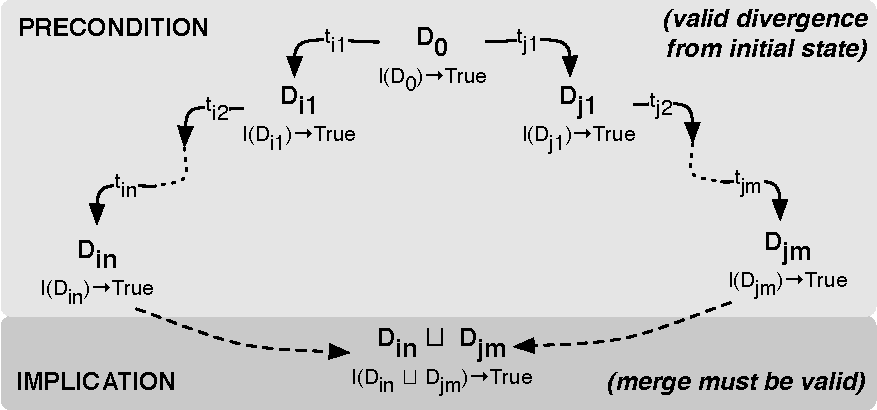
\includegraphics[width=\columnwidth]{figs/icommute.pdf}\vspace{-1em}
\end{center}
\caption{The \iconfluence property illustrated via a diamond
  diagram. If a set of transactions $T$ is \iconfluent, then all
  database states ($D_{in}$, $D_{jm}$) produced by $I$-valid sequences
  in $T$ starting from a common, $I$-valid database state ($D_s$) must
  be mergeable ($\sqcup$) into an $I$-valid database state.}
\label{fig:iconfluence}
\end{figure}

\subsection{\iconfluence and Coordination}

We can apply \iconfluence to our goals from Section~\ref{sec:model}:

\begin{theorem}
\label{theorem:necessary}
A globally $I$-valid system can execute transactions $T$ with
\cfreedom, transactional availability, convergence if and only if $T$
are \iconfluent with respect to $I$.
\end{theorem}

Theorem~\ref{theorem:necessary} establishes \iconfluence as a
necessary and sufficient condition for coordination-free
execution---the first such condition we are aware of. Effectively, we
have ``lifted'' the specification of semantics that are achievable
with scalability, availability, and low-latency to the abstraction of
invariants and transactions. If \iconfluence holds, these goals are
attainable; if not, there is no possible implementation or execution
strategy that can guarantee these properties for the provided
invariants and transactions. That is, if \iconfluence does not hold,
there exists at least one execution of transactions on divergent
replicas that will violate the given invariants when replicas
converge. To prevent invalid states from occurring, at least one of the
transaction sequences will have to forego availability or \cfreedom,
or the system will have to forego convergence. This is a useful
result, and we will spend much of the remainder of the paper applying
it.

Before doing so, we first prove Theorem~\ref{theorem:necessary}. The
forwards direction uses a partitioning argument~\cite{gilbert-cap} to
derive a contradiction, while the backwards direction is by
construction. Informally, if \iconfluence holds, each replica can
simply check each transaction's modifications locally and replicas can
simply merge independent modifications to guarantee convergence to a
valid state. For the converse, we construct a scenario under which a
replica cannot determine whether or not a non-\iconfluent update
should succeed without contacting another replica, diverging forever,
or compromising availability.\footnote{We can likely apply Newman's
  lemma and only consider single-transaction divergence (in the case
  of convergent and therefore ``terminating''
  executions)~\cite{obs-confluence,termrewriting}, but this is not
  necessary for our results.}

\begin{proof}{Theorem~\ref{theorem:necessary}}
($\Leftarrow$) We begin with the simpler proof, which is by
  construction. Assume a set of transactions $T$ are \iconfluent with
  respect to an invariant $I$. Consider a system in which each replica
  executes the transactions it receives against a copy of its current
  state and checks whether or not the resulting state is $I$-valid. If
  the resulting state is $I$-valid, the replica commits the
  transaction and its mutations to the state. If not, the replica
  aborts the transaction. Replicas asynchronously exchange copies of
  their local states and merge them. No individual replica will
  install an invalid state upon executing transactions, and, because
  $T$ is \iconfluent under $I$, the merge of any two $I$-valid replica
  states from individual replicas (i.e., valid sequences) as
  constructed above is $I$-valid. Therefore, the converged database
  state will be $I$-valid. Transactional availability, convergence,
  and global $I$-validity are all maintained via coordination-free
  execution.

($\Rightarrow$) Assume a system $M$ guarantees globally $I$-valid
  operation for set of transactions $T$ and invariant $I$ with
  \cfreedom, transactional availability, and convergence, but $T$ is
  not $I$-confluent. Then there exists an $I$-valid sequence
  $D_s=S_0(D_0)$ of transactions in $T$ and valid sequences $S_1,S_2$
  in $T$ such that $I(S_1(D_s)) \wedge I(S_2(D_s)) = true$
  but $I(S_1(D_s) \sqcup I(S_2(D_s)) = false$.

  Consider an execution $\alpha_0$ with two replicas $R_1$ and $R_2$
  in which a client submits $S_0$ to $R_1$. To maintain transactional
  availability and convergence, $R_1$ must commit $S_0$ and, after
  some period of time, exchange writes with $R_2$. At the end of
  $\alpha_0$, $R_1$ and $R_2$ will both contain $D_s$. Next, we
  consider an execution $\alpha_1$ beginning after convergence in
  $\alpha_0$ in which one client $C_1$ submits the transactions from
  $S_1$ to a replica $R_1$. We also consider a second execution
  $\alpha_2$ also beginning after convergence in $\alpha_0$ in which a
  second client $C_2$ submits the transactions from $S_2$ to replica
  $R_2$. To preserve transactional availability, in $\alpha_1$, $R_1$
  must commit the transactions in $S_1$ (resulting in $S_1(D_s)$),
  while, in $\alpha_2$, $R_2$ must commit the transactions in $S_2$
  (resulting in $S_2(D_s)$).

   We now consider a third execution, $\alpha_3$ to produce a
   contradiction. In $\alpha_3$, which begins immediately after
   convergence in $\alpha_0$, $C_1$ submits $S_1$ at exactly the same
   time as $C_2$ submits $S_2$; in our system model, $C_1$ and $C_2$
   will necessarily access different replicas because their operations
   are concurrently executing. $M$ is \cfree, so, from the perspective
   of $R_1$, $\alpha_3$ is indistinguishable from $\alpha_1$, and,
   from the perspective of $R_2$, $\alpha_3$ is indistinguishable from
   $\alpha_2$. However, if $R_1$ and $R_2$ each commit their
   respective sequences (as is required for transactional availability
   in $\alpha_1$ and $\alpha_2$), then their resulting states will, by
   assumption, not be $I$-valid under merge. Therefore, to preserve
   transactional availability, $M$ must sacrifice one of global
   validity (by allowing the invalid merge), convergence (by never
   merging), or \cfreedom (by forcing $R_1$ and $R_2$ to communicate
   prior to commit time).
\end{proof}

\subsection{Discussion}

\iconfluence captures a simple (informal) rule: \textbf{coordination
  can only be avoided if all local commit decisions are globally
  valid} (i.e. the merged global state satisfies all invariants). If
two independent decisions to commit can result in invalid converged
state, then replicas must coordinate in order to ensure that only one
of the decisions is to commit. If two such decisions exist, it is
unsafe for those operations to proceed in parallel, without
coordination. Given the existence of an unsafe execution and the
inability to distinguish between safe and invalid executions using
only local information, a globally valid system \textit{must}
coordinate in order to prevent the invalid execution.

\iconfluence analysis effectively captures points of \textit{unsafe
  non-determinism} in transaction execution. Total non-determinism, as
we have seen in many of our examples thus far, can compromise
application-level consistency. But not all non-determinism is bad: in
many cases, allowing concurrency necessarily entails allowing
non-determinism. \iconfluence analysis allows (non-deterministic)
divergence of database states but makes two powerful guarantees about
those states. First, the requirement for global validity ensures
safety (in the form of invariants). Second, the requirement for
convergence ensures liveness (in the form of
convergence). Accordingly, via its use of invariants, \iconfluence
allows users to scope non-determinism while permitting only those
(intermediate states and) outcomes that are
acceptable~\cite{consistency-borders}.

In contrast, a requirement for total determinism (e.g., ensuring
equivalent outcomes despite transaction execution order; in the
context of term-rewriting systems, \textit{confluence}) undoubtedly
aids in ease of programmability and
debugging~\cite{blooml,calm,termrewriting} but is too heavyweight of a
correctness criterion for many applications. As a classic example,
serializability is non-deterministic at the level of database state
because the final state may depend on the serial order that the system
chooses. (The consensus problem exhibits a similar requirement: a
value must be chosen, but \textit{which} value is not specified; a
requirement for non-determinism is often referred to as
non-triviality~\cite{paxos-commit}.) Perhaps more importantly, ensuring
deterministic outcomes does not necessarily guarantee
application-level consistency (safety): there is no guarantee that the
program outcome will obey invariants.

The use of invariants in \iconfluence allows greater precision in
analysis. We discuss specific trade-offs in
Section~\ref{sec:relatedwork}, but this definition is more general
than related concepts like state-based
commutativity~\cite{weihl-thesis} (e.g., equivalence of return values)
or confluence, as above. For example, in Lamport's example from
Section~\ref{sec:motivation}, the outcome of audit transactions
differs depend on whether it runs before or after a given deposit
transaction and is therefore not commutative or confluent with respect
to deposit transactions. However, audit transactions and deposit
transactions are indeed confluent with respect to the invariant that
the database does not contain negative account balances. Reasoning
about invariants instead of equivalence of database states is key to
achieving a \textit{necessary} and sufficient condition (instead of
simply a sufficient condition).




\section{Theory to Practice}
\label{sec:bcc-practice}

---

Conway's Law: combinations of operations and invariants commute: e.g., all write, no read, all read, no write

----

Applying analysis to systems:

Building a custom language is exciting but ultimately has performance challenges

Today, most immediate impact: programmers can manually reason about their application constraints without thinking about low-level models like causality and eventual consistency; also, smarter datatypes in the database like commutative counters and so on...

Low bar for a ``BCC'' system: each sp invocation (transaction) comes annotated with labels for either commuting or, if not, next hop in cycle (it's possible to collapse hops, but not strictly necessary); DB still doesn't know anything about stored procedures or integrity constraints

High bar for ``BCC'' system: all sp known in advance, all integrity contstraints know in advance

Our prototype focuses on the low bar for now---the high bar ventures into the domain of specialized program analysis. As we discuss in FUTUREWORK, we've had success in building small languages to capture the requirements of EVALUATION but reserve a full discussion for future work.

---

Merge function

There are some dumb answers: merge = nil; merge = LHS

Some better answers:
``bag'' semantics, expose all versions -- hard for the programmer, but effectively what ``immutability'' argument is all about

---

What commutes?

for now, assume we have data types that are known in advance: blobs/strings, numbers, counters

assume: PKEY, FKEY, UNIQUE, AUTOINCREMENT, NOGAP, !=, <, >

COMMUTES: 

counter.inc() and >
counter.dec() and <

any kind of !=
FKEY

with nonce, PKEY insert without specifying key
AUTOINCREMENT not sequential

CONFLICTS:

AUTOINCREMENT with NOGAP (sequential)
counter.inc() and <
counter.dec() and >
DELETE and insert into FKEY column


DISCUSSION: not claiming completeness (at this point), but, for a
simple SQL-like interface, this is actually pretty easy to enumerate
and, for simple programs, check. recursive SQL and unbounded loops
face the same problems, but, for the queries we've looked at, not
horrible.

---
When are different models useful?

Reads-from: FKey constraints
Atomic multi-put: FKey constraints

Uniqueness: nonce generators
RYW: sticky available

unavailability:
recency guarantees: deadlines (in a HA sense)
linearizability: breaking update cycles

---
How does this relate to more ad-hoc techniques?

Escrow: similar to a rely-guarantee from those PL guys--amortize
communication in exchange for unavailability during boundary
conditions/rebalancing

Immutability: makes merge trivial (if you solve the naming issue!);
says Gray: reads are writes

CRDTs/CALM: guarantee deterministic convergence to reasonable value;
weak safety guarantees (e.g., garbage is not returned [cite THINAIR])
but otherwise not safe for general purpose reads; Bloom\^L allows
'peek' but violates monotonicity



\section{Minding the Gap}
\label{sec:evaluation}

If achievable, coordination-freedom enables scalability limited to
that of available hardware: namely, server and network capacity. This
is powerful: a \cfree application can scale out without sacrificing
correctness, latency, or availability. In
Section~\ref{sec:bcc-practice}, we saw how many combinations of
invariants and transactions were not \iconfluent and how others were
not; in this section, we examine the implications of these results.

We begin by looking at the real-world costs of coordination: what
happens if \iconfluence does not hold? We quantify upper bounds on
throughput under common network delays. We next examine several
applications to understand whether their transactions are
implementable in a \cfree manner. We first focus on the current
standard for transactional performance---the TPC-C benchmark---and
show---both via \iconfluence analysis and by linearly scaling a
proof-of-concept implementation on public cloud infrastructure---that,
in contrast with classic, coordination-intensive execution strategies,
it is indeed achievable without distributed coordination. We next
examine several other benchmarks as recently proposed in the
literature~\cite{oltpbench} and discuss the implications of these
results on \cfreedom in real world deployments.

\subsection{Costs of Coordination}

\begin{figure}
  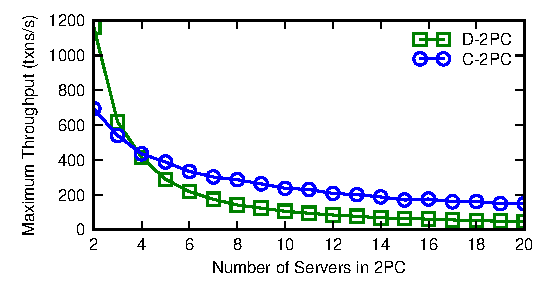
\includegraphics[width=\columnwidth]{figs/singledc-twopc.pdf}\\ {\centering
    \textbf{\scriptsize a.) Local-area network scenario based on
      traces from~\cite{bobtail}}\par}
  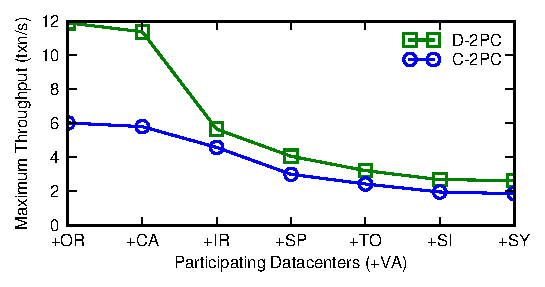
\includegraphics[width=\columnwidth]{figs/multidc-twopc.pdf}\\ \textbf{\scriptsize
    b.) Wide-area network scenario based on traces
    from~\cite{hat-vldb} with transactions origininating from a
    coordinator in VA (VA:~Virginia, OR:~Oregon, CA:~California,
    IR:~Ireland, SP:~S\~{a}o Paulo, TO:~Tokyo, SI:~Singapore,
    SY:~Sydney)}

\caption{Atomic commitment latency as an upper bound on throughput
  over LAN and WAN networks.}
\label{fig:2pc}
\end{figure}

What happens if a system must coordinate? One of the primary
challenges in scaling non-\cfree transactions is the atomic commitment
problem: if a given transaction might abort, all servers it accesses
(whether replicas of the same item or replicas of different items)
must agree to unilaterally commit or abort the
transaction~\cite{bernstein-book}. For example, in a serializable
database system, a system might check for read-write conflicts and
abort a transaction if any are found. In a coordination-avoiding
system, a system will have to check that non-\iconfluent transactions
do not execute concurrently and violate a given invariant (i.e.,
requiring mutual exclusion during commitment). This \textit{atomic
  commitment} problem is well studied in both the database and
distributed systems literature, with many
variants~\cite{atomictransactions,paxos-commit,traiger-tods} and poses
a scalability limitation because its latency limits
throughput. Indeed, multiple atomic commitment rounds can often
proceed in parallel (e.g., any two \iconfluent transactions can
independently commit), but, at the granularity of a single record
(i.e., a worst-case scenario), atomic commitment becomes a
bottleneck. There are many possible optimizations including batching
and reordering of commits~\cite{calvin}, but, for arbitrary schedules
of transactions, atomic commitment induces an upper bound on per-item
throughput for conflicting operations.

We performed a simple analysis using recently published datasets of
real-world communication delay from both local-area~\cite{bobtail} and
wide-area~\cite{hat-vldb} networks. We used Monte Carlo analysis to
simulate both traditional two-phase commit (using a coordinator, two
delays of $N$ messages each)~\cite{bernstein-book} (\cpc) and
decentralized two-phase commit (without a coordinator, one delay of
$N^2$ messages)~\cite{paxos-commit} (\dpc), assuming perfect
pipelining (i.e., send \texttt{prepared} immediately after
\texttt{commit}, with no aborts) and only considering network latency
(i.e., local processing time due to locking, latching, validation, or
I/O delays would only increase latency).

Figure~\ref{fig:2pc} show our results for both local-area
(\ref{fig:2pc}a) and wide-area (\ref{fig:2pc}b) networks.  In the
local area, with only two servers participating in atomic commitment
(e.g., replication factor of $2$ or, alternatively, two conflicting
operations on items residing on different servers), we see a maximum
attainable throughput of approximately $1100$ transactions per second
(via \dpc; $750$/s via \cpc). With ten servers participating, \dpc
throughput drops to only $120$ transactions per second (resp. $200$
for \cpc): the long-tail of network latency surfaces as the number of
messages sent increases. In the wide area, the effects are stark: if
only coordinating within the continental US from Virginia to Oregon,
\dpc message delays incur a latency of approximately $83$~ms per
commit, resulting in a throughput of $12$ operations per second. If
coordinating between all eight EC2 availability zones, throughput
drops to slightly over $2$ transaction per second in both algorithms.

While this study is based solely on reported latencies, deployment
reports corroborate our findings. For example, Google's F1 uses
optimistic concurrency control via WAN with commit latencies of $50$
to $150$~ms. As the authors discuss, this limits throughput to between
$6$ to $20$ transactions per second per data
item~\cite{f1}. Megastore's average write latencies of $100$ to
$400$~ms suggest similar throughputs to those that we have
predicted~\cite{megastore}. Again, \textit{aggregate} throughput may
be greater as multiple 2PC rounds for disjoint sets of data items may
safely proceed in parallel. However, \textit{worst-case} access
patterns will indeed greatly limit scalability.

\subsection{Proof of Concept}

If \cfree execution makes scaling easy and, as the prior section
showed, non-\iconfluent operation is expensive, where do real
applications fall in the spectrum? We discuss several in the next
section but, here, as proof of concept application of \cfreedom
analysis, we perform a brief case study of the classic benchmark for
OLTP performance. The TPC-C benchmark is often used as the gold
standard for database concurrency control~\cite{oltpbench} both in
research and in industry~\cite{tpcc}, and in recent years has been
used as a yardstick for distributed database
performance~\cite{calvin,hstore,silo}: how much coordination does
TPC-C require? As we show, little.

TPC-C requires the maintenance of twelve ``consistency criteria,'' or
invariants during the processing of transactions representing business
activities of a wholesale supplier. In light of our analysis from
Section~\ref{sec:bcc-practice}, none is particularly challenging;
space constraints prohibit a full discussion, but we sketch relevant
constraints and execution strategies below:
\begin{itemize}

\item \textit{Foreign key constraints (Consistency Constraints
  3.3.2.\{4-7, 11\}).} When a customer places a new order, the order
  is recorded in the \texttt{ORDER} table and corresponding entries
  for each item in the order should be recorded in the
  \texttt{ORDER-LINE} table. Similarly, the new order's ID should
  appear in the \texttt{NEW-ORDER} table. In a traditional database
  system, we might use locks to atomically control the visibility of
  these updates to multiple tables. However, our earlier analysis
  tells us that we can maintain these foreign key constraints under
  insert with \cfreedom. Indeed, with the newly proposed ANON
  algorithm~\cite{ramp-txns}, we can enforce these invariants without
  synchronous coordination.

\item \textit{Sequential ID assignment (Consistency Constraints
  3.3.2.2-3).} Each new order placed in each warehouse's ten districts
  requires a sequentially assigned ID (e.g.,
  \texttt{AUTO\_INCREMENT}). This poses a challenge: the
  \texttt{DISTRICT\_NEXT\_O\_ID} column must be incremented at the
  same time that corresponding rows are inserted into the
  \texttt{ORDER}, \texttt{NEW-ORDER}, and \texttt{ORDER-LINE}
  tables. From Section~\ref{sec:bcc-practice}, this sequential
  assignment is not \cfree, so, for compliant execution, we will need
  to coordinate (others ignore these constraints~\cite{hat-vldb,silo}
  at the expense of compliance). A traditional approach would hold
  locks for the duration of each transaction, but this greatly reduces
  throughput~\cite{abadi-vll}. Instead, a coordination-avoiding
  strategy can wait to assign the next ID until commit time. When
  inserting rows into the order tables, the database assigns the order
  a temporary, uniquely generated ID and, upon commit, updates a
  reference (in a separate table) that maps this temporary ID to point
  to the true sequential ID. (A similar process can be performed for
  deletion during order delivery.) Accordingly, the database only
  holds locks for a single atomic increment of the district ID
  counter.

\item \textit{Materialized view maintenance (Consistency Constraints
  3.3.2.\{1, 8-10, 12\})}. Throughout transaction execution, a variety
  of materialized counters should be maintained (e.g., \texttt{W\_YTD
    = sum(D\_YTD})). With appropriate counter data types as in
  Section~\ref{sec:merge} and the ANON algorithm above, these
  constraints are all achievable with \cfreedom.
\end{itemize}

All told, only two of TPC-C's invariants fail the \iconfluence test,
and, under standard partitioning strategies~\cite{calvin,schism}, this
synchronous coordination can be limited to a non-abortable, atomic
increment-and-get operation on each district's order sequence number
(on a single server). Our \cfreedom analysis shows that the remaining
ten invariants are achievable without synchronous coordination and the
remainder (3.3.2.2-3) are satisfiable via non-abortable single-site
operation. Indeed, when we execute the above query plan for backbone
of and the only distributed transaction in the workload (New-Order, as
focused on in~\cite{calvin}) on a linearizable, main-memory database
prototype (Figure~\ref{fig:clients}; we disregard think time and
per-warehouse client limits, as is
standard~\cite{calvin,hstore,abadi-vll,jones-dtxn}), we indeed
bottleneck on sequence number assignment. On EC2 \texttt{cr1.8xlarge}
instances, as depicted, we achieve over $12K$ New-Order transactions
per second per warehouse. Deploying multiple warehouses per server
decreases contention and we attain throughput in excess of $17K$
transactions per second before bottlenecking on CPU. There is no
synchronous coordination across servers, so varying the percentage of
distributed transactions results in a modest ($25\%$) throughput
reduction due to CPU utilization due to serialization and the OS
kernel's TCP/IP stack (Figure~\ref{fig:pct}). In contrast, traditional
(serializable) approaches (as Figure~\ref{fig:2pc} hints) incur
throughput overheads ranging from 66--88\%~\cite{abadi-vll}.

\begin{figure}
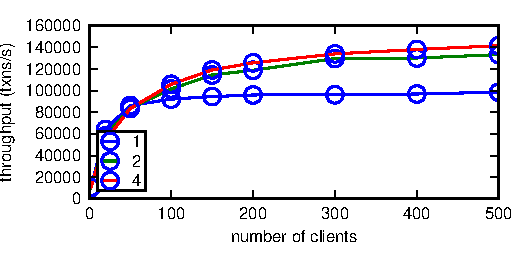
\includegraphics[width=\columnwidth]{figs/wh_thru.pdf}\vspace{-1em}
%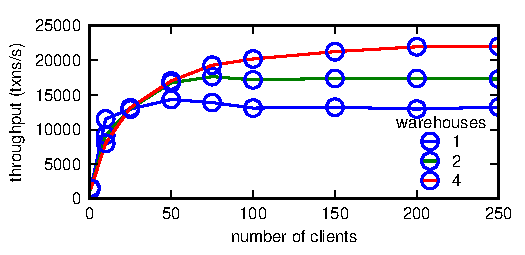
\includegraphics[width=\columnwidth]{figs/wh_thru_single.pdf}
\caption{TPC-C New-Order throughput across eight servers.}
\label{fig:clients}
\end{figure}

\begin{figure}
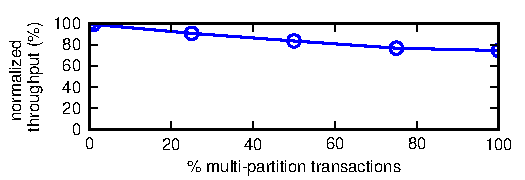
\includegraphics[width=\columnwidth]{figs/pct_thru.pdf}\vspace{-1em}
\caption{Coordination-free distributed execution of TPC-C New-Order
  (primary cost: CPU overhead due to serialization).}
\label{fig:pct}
\end{figure}

Unsurprisingly, a coordination-avoiding strategy allows linear scaling
(Figure~\ref{fig:scaleout}). On 100 EC2 \texttt{cc2.8xlarge} servers
in three \texttt{us-west} availability zones ($5$ warehouses per
server), we achieve over 1.6 million New-Order transactions per
second. We achieve 89.5\% of perfect scaling from one to 100 machines
and perfect scaling from ten to 100 machines. At peak, each server is
CPU bound due to our current, admittedly fairly inefficient
implementation. Nonetheless, by avoiding distributed coordination, we
can scale out. A comparison with a system providing serializability or
even Snapshot Isolation would be unfair, but we are unaware of any
other compliant TPC-C implementation that achieves greater than $500K$
New-Order transactions per second (e.g., Oracle 11G,
Calvin~\cite{calvin}, Silo's non-FastIDs~\cite{silo},
VLL~\cite{abadi-vll}). In contrast, we present these results as a
proof of concept that executing even ``challenging'' workloads like
TPC-C that contain many complex integrity constraints are not at odds
with scalability if implemented in a coordination-avoiding manner.

\begin{figure}
\begin{center}
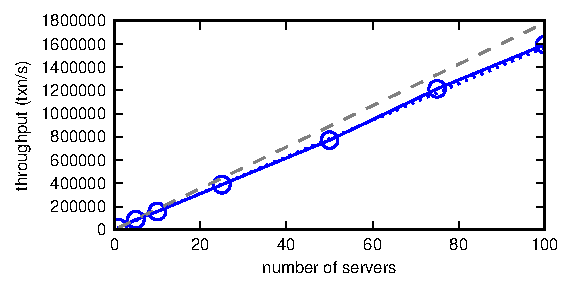
\includegraphics[width=\columnwidth]{figs/thru_scale.pdf}\vspace{-2em}
\end{center}
\caption{Coordination-free distributed execution of TPC-C New-Order is
  linearly scalable (dashed line is perfect scaling).}
\label{fig:scaleout}
\end{figure}

\minihead{Additional transactions} However, the remainder of the TPC-C
transactions are not distributed and are uninteresting: all operations
except for the Delivery transaction are implementable via a
combination of foreign key updates and commutative counter
increment/decrement, and the Delivery transaction is easily
implemented (as acknowledged in the benchmark
specification~\cite{tpcc}) as a single-partition transaction. The
TPC-C isolation requirements (reflecting the ANSI SQL specification)
are all achievable via client-side caching~\cite{hat-vldb}.

\subsection{Discussion}

These results begin to quantify the effects of coordination-avoiding
concurrency control. When conflicts cannot be avoided, coordination
(and atomic commitment can be expensive). However, if considering
\textit{application-level} invariants, databases only have to pay the
price of coordination when it is necessary. We were surprised that
this application-specific property was so favorable on the ``current
industry standard for evaluating the performance of OLTP
systems''~\cite{oltpbench}, but we are also aware that TPC-C may be a
simplification of real-world workloads.

For greater variety, we examined the transactions in the OLTPBenchmark
suite~\cite{oltpbench} and found (and confirmed with an author
of~\cite{oltpbench}) that, nine of fourteen remaining (non TPC-C)
benchmarks, the workload transactions did not involve integrity
constraints (e.g., did not modify primary key columns), one
(\texttt{CH-bencCHmark}) matched TPC-C, and two specifications implied
(but did not explicitly state) a requirement for coordination due to
unique ID assignment (\texttt{AuctionMark}'s \texttt{new-purchase},
\texttt{SEATS}'s \texttt{NewReservation}; achievable like TPC-C ID
assignment). The remaining two benchmarks, \texttt{sibench} and
\texttt{smallbank} were specifically designed as research benchmarks
for serializable isolation. The three ``consistency conditions'' in
the newer TPC-E benchmark (not in the prior suite) represent a subset
of the twelve conditions from TPC-C considered here (all materialized
counters). It is possible (even likely) that these benchmarks are
simply under-specified, but, according to official specification,
TPC-C contains the most rigorous coordination-intensive invariants
among the benchmarks we encountered.

Anecdotally, our conversations with end-users have not identified
invariants that are radically different than those we have proposed,
and a simple thought experiment identifying the invariants required
for, say, a social networking site, are fairly simple (e.g., username
uniqueness, foreign key constraints between updates, privacy
settings~\cite{pnuts}). Nonetheless, we view the further study of
real-world invariants to be a necessary area for future
investigation. In the interim, these preliminary results hint at what
is possible with coordination-avoidance as well as the costs of
coordination if \cfreedom is unachievable.





\section{Related Work}
\label{sec:relatedwork}

The research literature has a long tradition of using semantic
information in concurrency control for improved performance,
scalability, and availability.

% integrity constraints predate serializability; references here for
% substantial work on rewriting, maintaining, and minimizing
% computation cost for given integrity constraints-- our focus here is
% on semantics that can be achieved without coordination. our focus
% here is on replicated, non-atomic transactions.

\minihead{Integrity constraints} Use of integrity constraints in
database systems dates to at least 1974~\cite{florentin-constraints}
and has been studied extensively (see \cite{tamer-book} for an
summary). As~\cite{ic-survey,ic-survey-two} survey, a large body of
work examines how to perform query rewriting, transaction analysis,
and database design to accommodate a range of integrity
constraints. As \"{O}zsu and Valduriez~\cite{tamer-book} discuss, this
work largely presumes single-node databases (i.e., atomic---and
therefore non-\cfree---updates to shared state) and/or the use of
global concurrency control (for both prevention- and detection-based
approaches). Notably,~\cite{local-verification} avoids global
concurrency control and studies the problem of verifying constraints
in a shared-nothing, partitioned (but non-replicated) database
system. Our goal in this paper is to determine when we can avoid
global concurrency control and any coordination between
replicas. However, for non-coordination-free operations, this sizeable
body of literature provides a useful repository of techniques,
particularly given the increased cost of coordination in a replicated
environment.

% following serializability, looked at semantics for concurrency
% control

\minihead{Semantics-based Concurrency Control} A related body of
research similarly re-defines correctness criteria for shared
databases according to semantic definitions. \"{O}zsu and
Valduriez~\cite{tamer-book} also provide a brief summary of this work,
which, again, largely focuses on global (i.e., atomic, serializable,
or single-site) concurrency control strategies, but we discuss several
notable approaches here.

Much of semantics-based concurrency control uses application semantics
as a means to reduce conflicts during validation or execution of
concrete schedules of transactions (at
runtime)~\cite{badrinath-semantics} (i.e., via commutativity
analysis~\cite{weihl-thesis} or serial dependency
relations~\cite{herlihy-apologizing}). This prior work is eminently
useful when, indeed, conflicts are possible. However, this validation
(and conflict detection) requires communication between processes to
reach commit decisions. We instead seek to identify semantics that are
achievable entirely without coordination: \iconfluence analysis
statically reason about all \textit{possible} schedules of
transactions instead of performing run-time validation. If any two
operations can conflict, we flag them accordingly; run-time validation
of concrete schedules can indeed verify whether conflicts are present
by coordinating.

Several systems use application-provided labels as a means towards
determining when concurrent operations are safe. SDD-1~\cite{sdd1} and
Garcia-Molina~\cite{garciamolina-semantics}'s compatibility
  sets describe (manually-labeled) classes of transactions that can
be safely interleaved as a series of atomic steps (producing
``semantically consistent schedules''; equivalent to Korth's
predicate-wise
serializability~\cite{korth-serializability}). Bernstein and Lewis's
Assertional Concurrency Control~\cite{decomp-semantics}
furthers this analysis by leveraging axiomatic program analysis to
decompose transactions into a set of atomic steps and requiring
Hoare-style pre- and post-conditions for each individual
operation. Our \iconfluence reasons about divergent (non-atomic)
executions on multiple replicas but could be used to produce these
compatibility sets. Requring a single database-wide set of invariants
obviates the need for manually labeling transaction types.

Program decomposition via techniques like chopping~\cite{chopping}
(which is automatic), nested atomic
transactions~\cite{atomictransactions} (as in our sequence number
assignment of New-Order), and a range of alternate extended
  transaction models~\cite{acta} can further reduce conflicts once it
is established that invariant-based conflicts can actually occur.

\minihead{State-based Commutativity} Related work often reasons about
the commutativity of transaction \textit{outcomes}: for example, two
transactions provide state-based commutativity if their return value
is the same the the final state of the database is equivalent despite
reordering~\cite{weihl-data,weihl-thesis}. This state-based
commutativity is a sufficient but not necessary condition for
concurrent execution. Despite its conservativity, these techniques
have been successfully applied in diverse fields including both
database concurrency control and, recently, operating systems
design~\cite{kohler-commutativity}. State-based commutativity analysis
does not require the specification of application-level invariants
but, as~\cite{kohler-commutativity} notes, is accordingly not
necessary for maintaining correctness for all (and often common)
applications~\cite{lamport-audit}.

\minihead{Term rewriting} Our use of \iconfluence is directly inspired
by the literature on term rewriting and constraint programming. An
\iconfluent rewrite system guarantees that arbitrary rule application
will not violate a given invariant~\cite{obs-confluence}. This
generalizes traditional Church-Rosser confluence, which ensures that
any series of rewrites results in the \textit{same}
output~\cite{termrewriting}. To map between database and rewrite
systems, we can treat transactions as rewrite rules, the initial state
of the database as the initial constraint state, and the database
merge operator as a constraint \textit{join} operator that is defined
for all database states. Unlike term rewriting systems, our \cfreedom
analysis reasons about finite but arbitrarily long sequences of
transactions: our ``derivations'' are not finite as long as new
transactions can be introduced. We have found this literature to be a
useful grounding for our own formalism and see further comparison to
rewriting systems as an interesting starting point for future
theoretical analysis. Similar rewrite system concepts---including
confluence~\cite{aiken-confluence}---have been successfully integrated
into active database systems~\cite{activedb-book} (e.g., triggers and
rule processing), although we are not familiar with a concept
analogous to \iconfluence in this literature.

\minihead{Program analysis} The problem of maintaining correctness
despite concurrent modification is well studied in the programming
languages community. In particular, \iconfluence condition is closely
related to Owicki-Gries interference
  freedom~\cite{owickigries}, whereby concurrent operations cannot
interfere with one another's preconditions for execution as well as
Lamport's monotone assertions~\cite{lamport-safety}. As
Bernstein and Lewis~\cite{decomp-semantics} and Agrawal et
al.~\cite{agarwal-consistency} demonstrate, much of this programming
language theory on axomatic decomposition of concurrent programs can
be successfully applied to transaction schedules, particularly when
users specify guard pre-conditions on each transaction's
operations. However, the program analysis community almost exclusively
considers atomic update to shared state (as is reasonable on a
multiprocessor system), so the techniques are not immediately portable
to a model with replicated state that may diverge, as we consider
here.

\minihead{Hoping and Apologizing} In this work, we have assumed that
database state should \textit{always} be consistent with respect to
invariants. This is not strictly necessary for many applications. In
fact, applications can often benefit from probabilistically or
numerically-bounded deviations from consistent
state~\cite{epsilon-divergence}. Similarly, users can execute
compensating transactions to account for concurrent behavior (e.g.,
Sagas~\cite{sagas})~\cite{ic-survey,ic-survey-two}. These are worthwhile
strategies if programmers are willing to reason about inconsistent
state or otherwise write this compensatory code; here,
we seek a solution that does not require this of programmers or
database systems.

\minihead{Liveness and Convergence} The CALM
Theorem~\cite{ameloot-calm} shows that monotonic logic results in
deterministic program outcomes despite message re-ordering. Subsequent
program analysis in the Bloom~\cite{calm},
Bloom\textsuperscript{L}~\cite{blooml}, and Blazes~\cite{blazes}
languages statically highlight non-monotonic, non-confluent
operations. This is a useful \textit{liveness} guarantee---something
good will happen~\cite{lamport-safety}---but does not prevent users
from observing inconsistent database state---\textit{safety}, in the
form of application-level integrity constraints.  Here, we wish to
provide stronger guarantees (including safety) \textit{during
  execution}. In doing so, we relax the requirement that quiescent
database state be deterministic; we only require that it maintain the
specified application-level invariants (liveness). Similarly,
Commutative Replicated Data Type (CRDT) objects~\cite{crdt} ensure
that, once a database quiesces writes and all servers exchange writes,
the database will reflect all prior updates made to each CRDT. CRDTs
are accordingly useful in merging divergent replicas on a per-item
basis but do not solve the problem of maintaining application-level
consistency.

\minihead{High Availability and Scalability} A large class of systems
seeks to provide availability via ``optimistic
replication''~\cite{optimistic}, which, in the sense of Gilbert and
Lynch's CAP Theorem~\cite{gilbert-cap}, is equivalent to our goals of
coordination-freedom. \cite{hat-vldb} recently classified a range of
weak isolation and data consistency models according to their
availability via a range of proof-of-concept and informal, per-model
proofs. While we are inspired by this prior work, it did not consider
conditions for achieving application-level consistency and instead
focused on low-level read/write isolation anomalies. Towards more
practical systems, a range of stores such as SwiftCloud~\cite{swift}
often provide weak isolation, while related work on Red-Blue
Consistency~\cite{redblue} aims to provide mixed eventually consistent
and linearizable operations within a single store. We view this
related work as complementary to ours: here, we seek an understanding
of \textit{when} coordination is necessary rather than an optimal
implementation of a given model. Towards an understanding of actual
degrees of contention, Johnson et al. have characterized the
communication patterns of transaction synchronization as well as their
impact on database design~\cite{shore-communication}. We currently
focus on all-or-nothing communication requirements, but their
observations form the basis of a more thorough treatment of
non-\iconfluent updates.




\section{Future Work}
\label{sec:discussion}

In this paper, we have focused on the problem of recognizing when it
is possible to avoid distributed coordination. Here, we discuss
extensions to our approaches and outline areas for future work.

\minihead{Avoiding conflicts} Once a conflicting set of transactions
is identified via \iconfluence analysis, how should the conflict be
avoided? Our system model is amenable to many standard techniques like
backwards validation from optimistic concurrency
control~\cite{bernstein-book,tamer-book}, but the optimal
strategy---as is standard in concurrency control---is
workload-dependent. This hints at an opportunity for ``query
planning'' for coordination avoidance. For example, in a
producer-consumer scenario with an invariant requiring exactly-once
consumption, there are multiple strategies for coordination: all
producers could coordinate, or all consumers, or a mix of the two. The
correct choice depends on the physical location, prevalence, and
distribution of the producing and consuming transactions. Revisiting
heuristics- and statistics-based query planning, specifically
targeting physical layout, choice of concurrency control, and recovery
appears worthwhile. While recent work has used intelligent
partitioning to reduce distributed coordination~\cite{schism}, we see
this as only one aspect of a larger optimization problem.

\minihead{Amortizing coordination} We have analyzed conflicts on a
per-transaction basis, but it is possible to amortize the overhead of
coordination across multiple transactions. For example, the Escrow
transaction method~\cite{escrow} reduces coordination by allocating a
``share'' of non-\iconfluent operations between multiple
processes. For example, in a bank application, a balance of $\$100$
might be divided between five servers, such that each server can
dispense $\$20$ without requiring coordination to enforce a
non-negative balance invariant (servers can coordinate to ``refresh''
supply~\cite{mdcc}). In the context of our \cfreedom analysis, this is
similar to limiting the branching factor of the execution trace to a
some finite factor. We do not attempt a further comparison here but
believe that adapting Escrow and alternative time-, versioned-, and
numerical- drift-based models~\cite{yu-conit} is a promising area for
future work.

\minihead{Future system design} Given our formal grounding and early
quantitative results, what is the appropriate architecture for future
coordination-avoiding databases? Users could express their invariants
in a high-level language like SQL and the system could in turn avoid
and resolve conflicts without their further involvement. Analysis
tools could automatically inform system's conflict resolution policies
as suggested above. We believe this is feasible in the near-term but,
in turn, raises several interesting design and engineering challenges:
for example, as new invariants are added, the system must ensure that
satisfiability is possible. While we have focused on SQL, we might
also consider the use of restricted, \iconfluent operators (e.g.,
Bloom\textsuperscript{L}~\cite{blooml}) and more data types.




\section{Conclusion}
\label{sec:conclusion}

ACID transactions and associated strong isolation levels dominated the
field of database concurrency control for decades, due in large part
to their ease of use and ability to automatically guarantee
application correctness criteria. However, this powerful abstraction
comes with a hefty cost: concurrent transactions must coordinate in
order to prevent read/write conflicts that could compromise
equivalence to a serial execution. At large scale and, increasingly,
in geo-replicated system deployments, the coordination costs
necessarily associated with these implementations produce significant
overheads in the form of penalties to throughput, latency, and
availability. In light of these trends, we developed a formal
framework, called \fullnameconfluence, in which application invariants
are used as a basis for determining if and when coordination is
strictly necessary to maintain correctness. With this framework, we
demonstrated that, in fact, many---but not all---common database
invariants and integrity constraints are actually achievable without
coordination. By applying these results to a range of actual
transactional workloads, we demonstrated an opportunity to avoid
coordination in many cases that traditional serializable mechanisms
would otherwise coordinate. The order-of-magnitude performance
improvements we demonstrated via coordination-avoiding concurrency
control strategies provide compelling evidence that invariant-based
coordination avoidance is a promising approach to meaningfully scaling
future data management systems.


\scriptsize
\bibliography{bcc} \bibliographystyle{abbrv}


\end{document}
